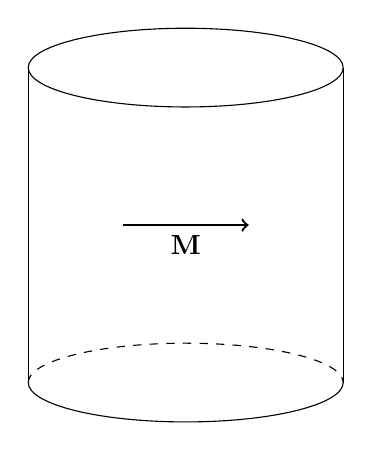
\begin{tikzpicture}
\def\leng {4}
\def\hgt {4}
\def\yrad {0.125}

% Draw cylinder
\draw (0,0.5*\hgt) circle [x radius = 0.5*\leng, y radius = \yrad*\leng];
\draw (-0.5*\leng,-0.5*\hgt) -- (-0.5*\leng,0.5*\hgt);
\draw (0.5*\leng,-0.5*\hgt) -- (0.5*\leng,0.5*\hgt);
\draw (-0.5*\leng,-0.5*\hgt) arc[x radius = 0.5*\leng, y radius = \yrad*\leng, start angle = -180, end angle = 0];
\draw[dashed] (-0.5*\leng,-0.5*\hgt) arc[x radius = 0.5*\leng, y radius = \yrad*\leng, start angle = 180, end angle = 0];

% Magnetisation vector
\draw[->,thick] (-0.2*\hgt,0) -- (0.2*\hgt,0) node[below,pos=0.5] {\(\mathbf{M}\)};

\end{tikzpicture}